\documentclass{article}

\begin{document}

\section{Introduzione allo strumento sviluppato}
\subsection{Motivazioni}
Lo strumento software sviluppato per questo lavoro di tesi ha lo scopo di automatizzare il processo di testing di vincoli per la già citata libreria JSetL. \\
Il linguaggio principale di implementazione è il C++, ma sono presenti anche parti di codice in Prolog e in Java. \\
Rifacendosi alla classificazione delle tipologie di testing illustrata nel capitolo 1, lo strumento si inserisce nella categoria di \emph{black-box} testing, ed in particolare nella sottocategoria \emph{boundary-value analysis} con criterio di input space partitioning \emph{all combinations}.\\
Per quanto riguarda le fasi del processo di testing, lo strumento si occupa in particolare di trattare la fase di \emph{unit testing}.\\
A differenza dei classici tool di generazione automatica di test, quello realizzato in questo lavoro di tesi è pensato specificatamente per JSetL: ciò permette di avere qualche vantaggio in più, come evidenziato di seguito.\\
JSetL è sostanzialmente l'implementazione Java del linguaggio \mathcal{L\textsubscript{\(\mathcal{BR}\)}}.\\
Esiste però, come citato in precedenza, anche un'analoga implementazione per il linguaggio Prolog, ossia \{log\}.\\
Il fatto di avere una doppia implementazione non è assolutamente banale per un sistema software, e per uno strumento che deve effettuarne il testing può rivelarsi un notevole punto di forza.\\
Un primo vantaggio è dato dal fatto che all'utente è richiesto solamente di specificare la forma che dovrà avere il test set, senza mai dover esplicitare il risultato di ogni test in anticipo (non è necessario sapere se un vincolo è o meno soddisfacibile). La soddisfacibilità è infatti \say{calcolata} dall'interprete \{log\}: lo strumento sfrutta \{log\} per ricavare i risultati dei singoli test (true o false), per poi riportarli (senza ricalcolarli) sui test JSetL.\\

\clearpage

In questo modo si ha un ulteriore vantaggio indiretto: un'eventuale incongruenza sul risultato di un test è subito visibile, in quanto la direttiva \emph{assert} corrispondente nel codice Java non andrebbe a buon fine.\\
Questa incongruenza è spesso un campanello d'allarme che può aiutare lo sviluppatore a capire se vi sono incoerenze tra le due implementazioni.\\

\clearpage

\subsection{Architettura del sistema}
L'architettura del sistema software sviluppato è descritta dal seguente schema.\\\\ 


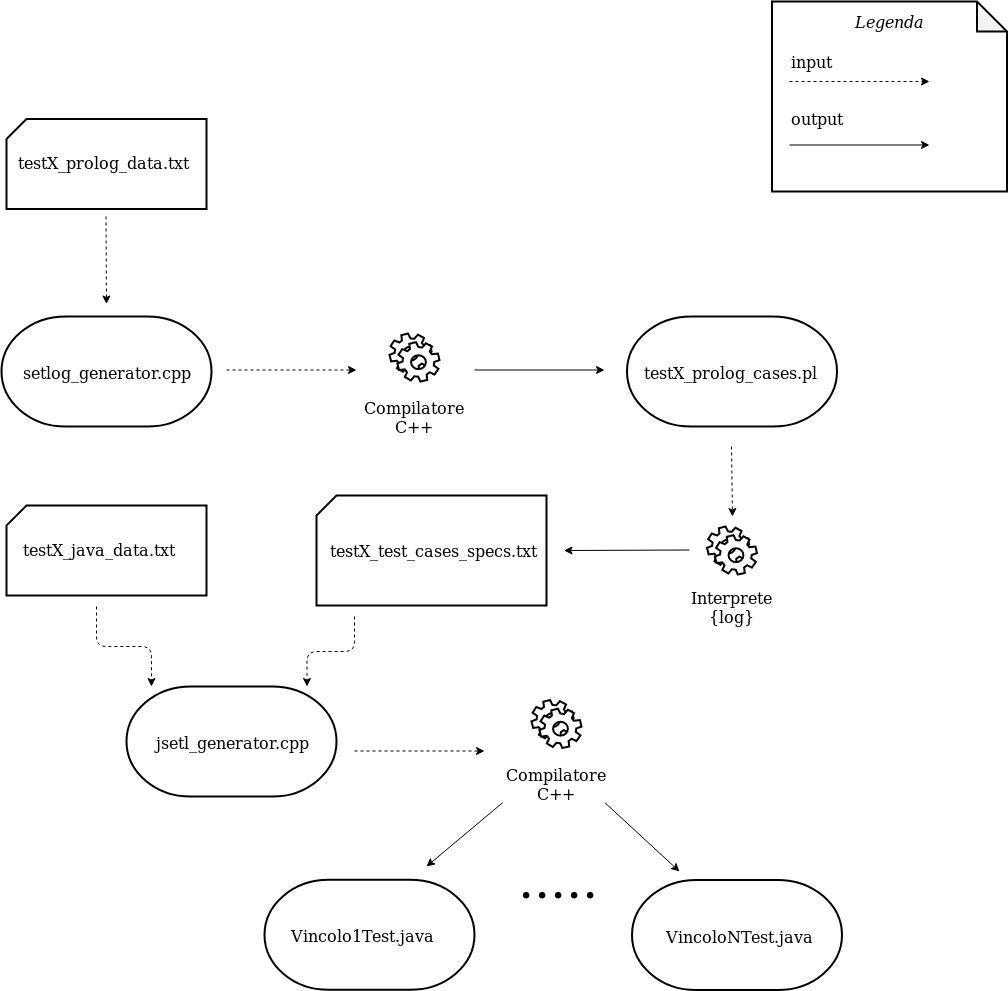
\includegraphics[scale=0.4]{images/architecture.png}
    

\clearpage

L'utente avvia il processo di generazione dei test fornendo in input al sistema due file: \texttt{testX\_prolog\_data.txt} e \texttt{testX\_java\_data.txt}.

I due file contengono le informazioni fondamentali sul test set che si intende generare, ossia quali sono i vincoli che si vogliono testare e su quali argomenti essi devono essere istanziati (per test set si intende una collezione di casi di test riferiti ad uno o più vincoli, dove ogni singolo caso è un test istanziato su una particolare combinazione degli argomenti).\\

\texttt{testX\_prolog\_data.txt} specifica questi vincoli e argomenti in sintassi \{log\}, mentre in \texttt{testX\_java\_data.txt} sono espressi in sintassi Java. \\
Il contenuto semantico dei due file è però identico: vincoli e argomenti devono essere uguali in numero e devono soprattutto mantenere il medesimo significato.\\
Una volta forniti questi due file di input, la cui sintassi sarà illustrata in seguito nel dettaglio, il processo di generazione può avere inizio.\\

Il programma \texttt{setlog\_generator.cpp} riceve in input il file \texttt{testX\_prolog\_data.txt}. \\
Una volta compilato, genera in output il file \texttt{testX\_prolog\_cases.pl}. \\
Quest'ultimo è un programma Prolog contenente il test di ogni vincolo su tutti i possibili argomenti specificati, ovviamente con sintassi \{log\}.\\

Il file \texttt{testX\_prolog\_cases.pl} viene quindi dato in input all'interprete \{log\}, che genererà in output il file \texttt{testX\_test\_cases\_specs.txt}. \\
Questo file testuale contiene una serie di record in cui vengono specificati il nome del vincolo, i suoi argomenti ed il risultato ottenuto tramite l'interprete \{log\} eseguendo quel particolare caso di test (true o false).\\

Quest'ultimo file ed il file \texttt{testX\_java\_data.txt} sono infine dati in input al programma \texttt{jsetl\_generator.cpp}, il quale genera in output $n$ classi Java (con $n$ $=$ numero di vincoli definiti nelle specifiche dall'utente).\\
Ogni classe Java si occupa quindi del test di un solo vincolo, e per ogni vincolo vengono generati i relativi metodi di test.\\
Gli argomenti su cui ogni metodo di test è istanziato sono ottenuti dal file \\ \texttt{testX\_java\_data.txt}, mentre il risultato del test (true o false) è ricavato dal file \texttt{testX\_test\_cases\_specs.txt}, ossia dai risultati generati dall'interprete \{log\}. \\

Durante l'esecuzione di \texttt{jsetl\_generator.cpp}, è inoltre richiesto all'utente se è interessato o meno ai tempi di esecuzione di ciascun vincolo. \\
Nel caso la risposta sia affermativa, ogni classe Java verrà integrata con una parte aggiuntiva di codice per permettere la stampa dei tempi di esecuzione su un file denominato \texttt{times.txt}.\\

Una volta ottenute le $n$ classi Java, è sufficiente caricarle nel proprio IDE Java, assicurarsi di avere disponibili sia JSetL che JUnit, e dare il comando \emph{"run as JUnit test"}.\\
Se la stampa dei tempi è stata abilitata, dopo aver dato questo comando verrà inoltre creato il file \texttt{times.txt}, in cui verrà aggiunto un record contenente il nome del vincolo appena testato con il relativo tempo di esecuzione espresso in millisecondi, calcolato come somma di tutti i tempi di esecuzione dei singoli metodi di test.\\

\newpage
\thispagestyle{empty}
\mbox{}

\end{document}